\section{Flanger}
The flanger effect gets its name from the original analog method of running two tape machines slightly out of sync with each other. It is based on the principle of contructive and destructive interference of signals.
A clear comprehension of the flanger from a perceptive point of view  is highlighted by the frequency response of the comb filter. 
At the heart of the algorithm, comb filter is the simplest example of recursive delay network.
In fact, flanger is a recursive comb filter with interpolating and time-varying delay line. Changes in delay time correspond to the characteristic way peaks in the frequency response move up and down in frequency\cite{puckette2006theory}.

Comb filter is obtained feeding a $g_{FB}$ fraction of the output back to the input as we can see looking at (figura) its typical difference equation:

\[
y[n] = g_{FB} y[n - M(n)] + x[n] + (g_{FF} - g_{FB}) x[n - M[n]],
\]
where $g_{FF}$ is the \textit{depth} of the flanger and $M[n]$ is a function describing variable delay times. In the case of interest it is represented by a Low Frequency Oscillator of different and selectable waveforms. Thus, the frequency response of the flanger is equal to 
\[
\frac{Y[z]}{X[z]} = \frac{1 + z^{-M[n]} (g_{FF} - g_{FB})} {1 - z^{-M[n]}  g_{FB} }
\]

and looking at the absolute value of the frequency response of the non-recirculating comb filter with $g_{FB} = 0$ 
\[
|H(z)| = \sqrt{ 1 + 2g_{FF} cos(\omega M[n]) + g_{FF}^1}
\]
we can appreciate the classical spectrum with peaks and notches lying respectively in 
\[
\omega_p = \frac{2 \pi p}{M},
\]
where $p = 0, 1, 2, ..., M-1$ and 
\[
\omega_n = \frac{(2n+1) \pi}{M},
\]
where $n = 0, 1, 2, ..., M-1$. Now, it is easy to see the dependence between frequencies enhanced and delay times of the flanger. 
\begin{figure}
	\centering
	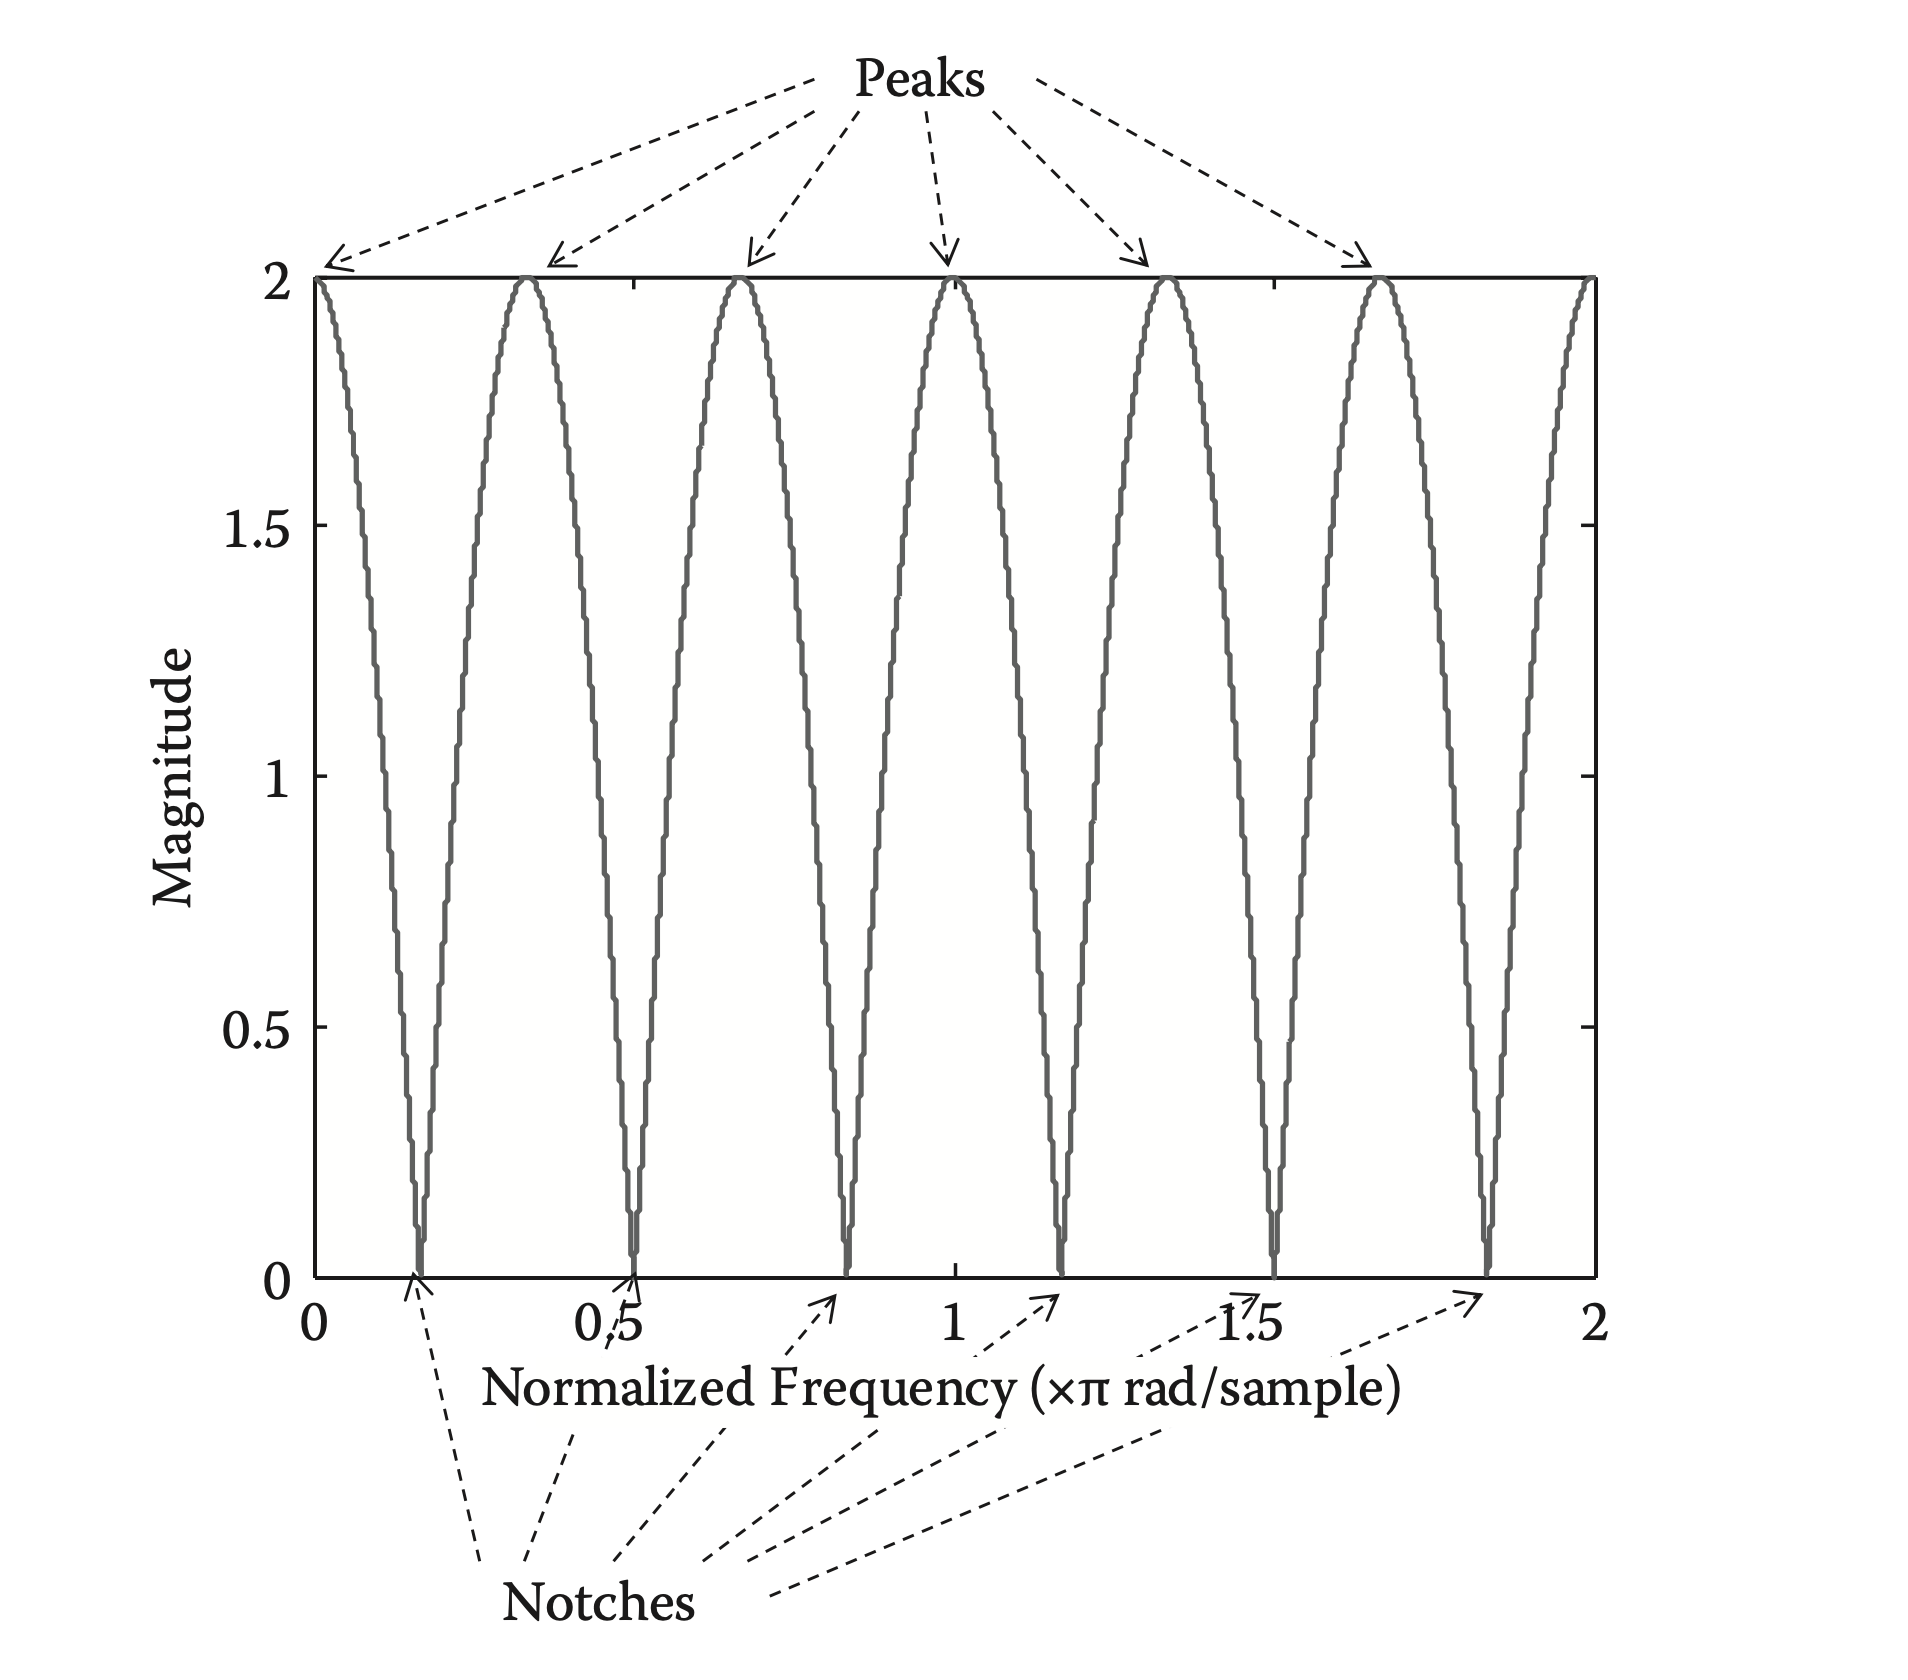
\includegraphics[width=0.5\linewidth]{assets/comb.png}
	\caption{Frequency response of a flanger.}
	\label{fig:comb}
\end{figure}

The flanger is stable until $g_{FB} < 1$. 
Our plug-in provides the feature to invert the polarity of the $g_{FF}$ parameter. In this case, peaks and notches in the frequency response will trade places and the first notch lies now at $DC$ frequency. Because of it, switching to the negative polarity you can hear a thinner sound unless $M$ is large.

In order to reproduce the analog effect of the flanger given by the heads of the tape machine, a delay line with a read and a writ pointer must be implemented. In the code we define them as two float variables dr and dw. The read index moves away from, then back to the top or starting point of the delay. When the read pointer and the write one are superimposed there is no delay, while when they are moving with respect to each other there is a change of pitch. This concept approaches the Doppler effect. As can be seen from the graph, the flanger effect is given precisely by the mix of the dry signal and the wet one(in fact if only the signal with modulated delay were sent out, we would have a sort of simple frequency modulation that would lead to a vibrato effect ). In short, mixing an audio signal with a slightly delayed copy of itself results in a different frequency spectrum due to the suppression of some wave components and the enhancement of others.\par
So the mixing ratio between the two signals is a fundamental aspect of this type of effect. The control of the \textbf{depth} value, expressed in percentage,is used to decide the amount of wet signal to mix to the dry one. In particular 0\% corresponds to g=0 and produces no effects, while 100\% guarantees the maximum effect.\\
Another free parameter for the user is the value of the \textbf{feedback gain}. It is expressed in percentage to. In particular from the graph it can be seen that setting this value equal to 0\% makes this flager match the basic one without feedback. We decided to set the range of this parameter from 0 to 99\% to remain in a stable condition and prevent the risk of distortion of the sound.\\
As said before, the delay line is controlled by an LFO. We decided to set other degree of freedom for the user and we introduced some other user-adjustable parameters related to it. In particular \textbf{sweep width} is the value of the amplitude of the LFO expressed in terms of number of samples, in a range from  0 to 25. It is also possible to modify the \textbf{LFO frequency}, from 0 to 10 Hz. This parameter is useful to act on the speed of the read pointer. The plugin also provides the possibility to choose the type of wave. Besides the default sine wave, it is possible to set a square, saw tooth, inverse saw tooth, triangular and random waves. This part of code is implemented with a simple switch in FlangerProcessor::waveForm.
We also add the possibility to change the polarity of the signal.

With high values of feedback gain and depth, we can occur in the risk of saturation (giusto?) in particular at low frequencies. In order to avoid that, we added an high pass filter in input to the wet signal line, implemented with the following formula:




